\documentclass[11pt,nocut]{article}

\usepackage{../latex_style/packages}
\usepackage{../latex_style/notations}
\externaldocument{../lecture_02/lecture_02}
\externaldocument{../lecture_04/lecture_04}


\title{\vspace{-2.0cm}%
	Optimization and Computational Linear Algebra for Data Science\\
Lecture 7: Singular value decomposition}
\author{Léo \textsc{Miolane} \ $\cdot$ \ \texttt{leo.miolane@gmail.com}}
\date{\today}

\begin{document}
\maketitle
\textbf{Warning:}
\emph{This material is not meant to be lecture notes. It only gathers the main concepts and results from the lecture, without any additional explanation, motivation, examples, figures...
}


\section{The Spectral Theorem}

The main result of this section is the following ``Spectral Theorem'' which tells us that a symmetric matrix is diagonalizable in an orthonormal basis.

\begin{theorem}[Spectral Theorem]\label{th:spectral}
	Let $A \in \R^{n \times n}$ be a \textbf{symmetric} matrix. Then there is a orthonormal basis of $\R^n$ composed of eigenvectors of $A$.
\end{theorem}

Given an $n \times n$ symmetric matrix $A$, Theorem \ref{th:spectral} tells us that one can find an orthonormal basis $(v_1, \dots, v_n)$ of $\R^n$ and scalars $\lambda_1, \dots, \lambda_n \in \R$ such that for all $i \in \{1, \dots, n\}$,
$$
A v_i = \lambda_i v_i.
$$
Let $P$ be the $n \times n$ matrix whose columns are $v_1, \dots, v_n$. Since $(v_1, \dots, v_n)$ is an orthonormal basis, we get that $P$ is an orthogonal matrix. Let $D = {\rm Diag}(\lambda_1, \dots, \lambda_n)$ and compute
$$
A P
= 
A 
\begin{pmatrix}
	| & | & & | \\
	v_1 & v_2 & \cdots& v_n \\
	| & | & & |
\end{pmatrix}
= 
\begin{pmatrix}
	| & | & & | \\
	Av_1 & Av_2 & \cdots& Av_n \\
	| & | & & |
\end{pmatrix}
= 
\begin{pmatrix}
	| & | & & | \\
	\lambda_1 v_1 & \lambda_2 v_2 & \cdots& \lambda_n v_n \\
	| & | & & |
\end{pmatrix}
= P D.
$$
By multiplying by $P^{\sT}$ on both sides, we get $A P P^{\sT} = P D P^{\sT}$. Recall now that $P$ is orthogonal, therefore $P P^{\sT} = \Id_n$. We conclude that $A = P D P^{\sT}$.

\begin{theorem}[Spectral Theorem, matrix formulation]\label{th:spectral2}
	Let $A \in \R^{n \times n}$ be a symmetric matrix. Then there exists an orthogonal matrix $P$ and a diagonal matrix $D$ of sizes $n \times n$, such that
	$$
	A = P D P^{\sT}.
	$$
\end{theorem}

\begin{proposition}\label{prop:eigen_var}
	Let $A$ be a $n \times n$ symmetric matrix and let $\lambda_1 \geq \cdots \geq \lambda_n$ be its $n$ eigenvalues and $v_1, \dots, v_n$ be the associated orthonormal family of eigenvectors. Then 
	$$
	v_1 = \argmax_{\|v\| = 1} v^{\sT} A v\,,
	\qquad \text{and for} \ k=2, \dots n, \qquad
	v_{k} = \argmax_{\|v\| = 1, \, v \perp v_1, \dots, v_{k-1}} v^{\sT} A v.
	$$
\end{proposition}

\begin{remark} Applying the proposition above to the matrix $-A$ which is symmetric with eigenvalues $-\lambda_n \geq \cdots \geq -\lambda_1$ and associated eigenvectors $v_n, \dots, v_1$, we get
	$$
	v_n = \argmin_{\|v\| = 1} v^{\sT} A v\,,
	\qquad \text{and for} \ k=1, \dots , n-1 \qquad
	v_{k} = \argmin_{\|v\| = 1, \, v \perp v_{k+1}, \dots, v_{n}} v^{\sT} A v.
	$$
\end{remark}

\subsection*{Positive matrices}

\begin{definition}
	A symmetric matrix $A \in \R^{n \times n}$ is said to be \emph{positive semi-definite} if 
	\begin{equation}\label{eq:def_pos}
		\forall x \in \R^n, \ x^{\sT} A x \geq 0.
	\end{equation}
	The matrix $A$ is said to be \emph{positive definite} if moreover the inequality in \eqref{eq:def_pos} is strict for all $x \neq 0$.
\end{definition}
\begin{remark}
	Negative semi-definite and negative definite matrices are defined analogously.
\end{remark}

\begin{proposition}
	Let $A \in \R^{n \times n}$ be a symmetric matrix, and let $\lambda_1, \dots,\lambda_n \in \R$ its eigenvalues. Then
	$$
	A \ \text{is positive semi-definite} \ \Longleftrightarrow \
	\lambda_i \geq 0 \ \text{for} \ i = 1, \dots, n,
	$$
	and
	$$
	A \ \text{is positive definite} \ \Longleftrightarrow \
	\lambda_i > 0 \ \text{for} \ i = 1, \dots, n.
	$$
\end{proposition}

\begin{exercise}
	Let $A \in \R^{n \times n}$.
	\begin{enumerate}[label=\alph*.]
		\item Show that $A^{\sT} A$ positive semi-definite.
		\item Let $M$ be a $n \times n$ symmetric positive semi-definite matrix. Show that there exists $A \in \R^{n \times n}$ such that $M = A^{\sT} A$.
	\end{enumerate}
\end{exercise}

\section{Singular value decomposition}

\begin{theorem}[Singular value decomposition (SVD)]\label{th:SVD}
	Let $A \in \R^{n \times m}$. Then there exists two orthogonal matrices $U \in \R^{n \times n}$ and $V \in \R^{m \times m}$ and a matrix $\Sigma \in \R^{n \times m}$ such that $\Sigma_{1,1} \geq \Sigma_{2,2}  \geq \cdots \geq 0$ and $\Sigma_{i,j} = 0$ for $i\neq j$
	$$
	A = U \Sigma V^{\sT}.
	$$
	The columns $u_1, \dots, u_n$ of $U$ (respectively the columns $v_1, \dots, v_m$ of $V$) are called the left (resp.\ right) singular vectors of $A$. The non-negative numbers $\Sigma_{i,i}$ are the singular values of $A$. Moreover $\rank(A) = \# \{i \, | \, \Sigma_{i,i} \neq 0 \}$.
\end{theorem}

Notice that the singular vectors (similarly to the eigenvectors) are not uniquely defined: if $A = U \Sigma V^{\sT}$ is a SVD of $A$, then $A = (-U) \Sigma (-V)^{\sT}$ is also a SVD of $A$. However, with a slight abuse of language, we will often refer $v_i$ as the $i^{\rm th}$ right singular vector of $A$.

\subsection{Properties of the SVD}

Let $A \in \R^{n \times m}$ and let $U \Sigma V^{\sT}$ be a singular value decomposition of $A$ as in Theorem \ref{th:SVD}. Let $u_1, \dots, u_n$ be the left singular vectors (i.e.\ the columns of $U$) and $v_1, \dots, v_m$ be the right singular vectors (i.e.\ the columns of $V$). Let $\sigma_i = \Sigma_{i,i}$ be the singular values of $A$.

\begin{proposition}
	For $i=1, \dots, \rank(A)$ we have
	$$
	A v_i = \sigma_i u_i
	\qquad \text{and} \qquad
	A^{\sT} u_i = \sigma_i v_i.
	$$
\end{proposition}

The most important property of the singular vectors for us is the following:
\begin{proposition}\label{prop:max_svd}
	We have
	\begin{equation}
		v_1 = \argmax_{\|v\| = 1} \|A v\| 
		\qquad \text{and} \qquad 
		\sigma_1 = \max_{\|v\| = 1} \|A v\|.
	\end{equation}
	It holds also that
	\begin{equation}
		v_2 = \argmax_{\|v\| = 1, \, v \perp v_1} \| A v \|
		\qquad \text{and} \qquad 
		\sigma_2 = \max_{\|v\| = 1, \, v \perp v_1} \| A v \|
	\end{equation}
	and more generally:
	\begin{equation}
		v_{k}   = \argmax_{\|v\| = 1, \, v \perp v_1, \dots, v_{k-1}} \| A v \|.
		\qquad \text{and} \qquad 
		\sigma_{k} = \max_{\|v\| = 1, \, v \perp v_1, \dots, v_{k-1}} \| A v \|.
	\end{equation}
\end{proposition}
\begin{remark}
	Considering $A^{\sT}$ leads to an analogous result for the left singular vectors $u_k$:
	\begin{equation}
		u_{k}   = \argmax_{\|u\| = 1, \, u \perp u_1, \dots, u_{k-1}} \| A^{\sT} u \|.
		\qquad \text{and} \qquad 
		\sigma_{k} = \max_{\|u\| = 1, \, u \perp u_1, \dots, u_{k-1}} \| A^{\sT} u \|.
	\end{equation}
\end{remark}
\begin{proof}
	Compute $A^{\sT} A = V \Sigma^{\sT} \Sigma V^{\sT} = V D V^{\sT}$ where the matrix $D \defeq \Sigma^{\sT} \Sigma$ is diagonal with $D_{i,i} = \sigma_i^2$. The family $(v_1, \dots, v_m)$ is therefore an orthonormal family of eigenvectors of the symmetric matrix $A^{\sT} A$ and $\sigma_1^2 \geq \cdot \geq \sigma_m^2$ are the corresponding eigenvalues. The result follows then from Proposition \ref{prop:eigen_var} applied to $A^{\sT} A$, noticing that $v^{\sT} A^{\sT} A v = \|Av\|^2$.
\end{proof}


\subsection{Proof of Theorem \ref{th:SVD}}
We apply the Spectral Theorem (Theorem \ref{th:spectral}) to the $m \times m$ matrix $A^{\sT} A$: there exists an orthonormal basis $(v_1, \dots, v_m)$ of $\R^m$ of eigenvectors of $A^{\sT} A$ associated to eigenvalues $\lambda_1 \geq \cdots \geq \lambda_m$ that are all non-negative because $A^{\sT} A$ is non-negative.
Let $V \in \R^{m \times m}$ be the orthogonal matrix whose columns are $(v_1, \dots, v_m)$.
\\

Let us write $\sigma_i = \sqrt{\lambda_i}$ and let $r = \max\{ i | \sigma_i > 0\}$.
Define for $i = 1, \dots, r$
\begin{equation}\label{eq:def_u}
	u_i = \frac{1}{\sigma_i} A v_i \in \R^n.
\end{equation}
\begin{lemma}
	The family $(u_1, \dots, u_r)$ is orthonormal.
\end{lemma}
\begin{proof}
	Let $i,j \in \{1, \dots, r \}$.
	$$
	\langle u_i, u_j \rangle = \Big(\frac{1}{\sigma_i} A v_i\Big)^{\sT}\Big(\frac{1}{\sigma_j} A v_j\Big) = \frac{1}{\sigma_i \sigma_j} v_i^{\sT} A^{\sT} A v_j
	= \frac{\sigma_i}{\sigma_j} v_i^{\sT} v_j = \1_{i = j},
	$$
	since $A^{\sT} A v_i = \sigma_i^2 v_i$.
\end{proof}

If $r < n$ we let $(u_{r+1}, \dots, u_n)$ be an orthonormal family of vectors of $\R^n$ that are orthogonal to $u_1, \dots, u_r$. The family $(u_1, \dots, u_n)$ is then an orthonormal basis of $\R^n$
Let $U \in \R^{n \times n}$ be the orthogonal matrix whose columns are $(u_1, \dots, u_n)$.

\begin{lemma}\label{lem:kernelA}
	For $i = r+1, \dots, m$, $A v_i = 0$.
\end{lemma}
\begin{proof}
	We compute for $i = r+1, \dots, m$:
	$$
	\|Av_i \|^2 = v_i^{\sT} A^{\sT} A^{\sT} v_i = v_i^{\sT}(\lambda_i v_i) = \sigma_i^2 = 0.
	$$
\end{proof}
\\

Finally, we let $\Sigma \in \R^{n \times m}$ defined by:
$$
\Sigma_{i,j} =
\begin{cases}
	\sigma_i & \text{if} \quad i=j \\
	0 & \text{otherwise}.
\end{cases}
$$
It remains to verify that $A = U \Sigma V^{\sT}$.
Compute for $i=1, \dots, m$, using the definition \eqref{eq:def_u} and Lemma \ref{lem:kernelA}:
$$
A v_i = 
\begin{cases}
	\sigma_i u_i & \text{if} \ i \leq r \\
	0 & \text{otherwise}.
\end{cases}
$$
By orthogonality of $V$ and the construction of $\Sigma$ one verifies easily that
$$
U \Sigma V^{\sT} v_i = 
\begin{cases}
	\sigma_i u_i & \text{if} \ i \leq r \\
	0 & \text{otherwise}.
\end{cases}
$$
We conclude that for all $i \in \{1, \dots, m\}$, $A v_i = U \Sigma V^{\sT} v_i$. Since a linear transformation is uniquely determined by the image of a basis, we conclude that $A = U \Sigma V^{\sT}$.
\\

It remains to show:
\begin{lemma}
	$\rank(A) = r$.
\end{lemma}
\begin{proof}
	The family $(u_1, \dots, u_r)$ is orthonormal, hence linearly independent. By definition $u_i \in \Im(A)$ which implies that $\rank(A) = \dim(\Im(A)) \geq r$.
	To prove the converse inequality, notice that by Lemma \ref{lem:kernelA} $v_i \in \Ker(A)$ for $i=r+1, \dots, m$.
	The vectors $(v_{r+1}, \dots, v_m)$ are orthonormal, hence linearly independent. This implies that $\dim(\Ker(A)) \geq m-r$. We conclude by applying the rank Theorem:
	$$
	\rank(A) = m - \dim(\Ker(A)) \leq m - (m-r) = r.
	$$
\end{proof}
\\

\section{Interpretation and applications of the SVD}

\subsection{Geometric interpretation}

\subsection{``Maximal variance'' interpretation}\label{sec:maximal_variance}
Let $a_1, \dots, a_n \in \R^d$ be $n$ points in $d$ dimensions. We assume that this points are centered, meaning that 
$$
\sum_{i=1}^n a_i = 0.
$$
Let $A$ be the $n \times d$ matrix whose rows are $a_1, \dots, a_n$ and let $(v_1, \dots, v_n)$ be its right singular vectors.
By Proposition \ref{prop:max_svd}, $v_1$, the first right singular vector of $A$, maximizes
$$
v \mapsto \|A v\|^2 =  \sum_{i=1}^n \langle a_i, v \rangle^2
$$
over the unit sphere.
This quantity is the variance of the coordinates of the points $a_1, \dots, a_n$ along the direction $\Span(v)$.

The first right singular vector $v_1$ gives therefore the direction along which the variance of the data is maximal. Proposition \ref{prop:max_svd} gives also that
\begin{equation}
	v_{k} = \argmax_{\|v\| = 1, \, v \perp v_1, \dots, v_{k-1}} \| A v \|^2.
\end{equation}
Hence $v_2$ gives the direction orthogonal to $v_1$ that maximizes the variance and so on...

\subsection{Application: Principal Component Analysis (PCA)}

The SVD is commonly used for dimensionality reduction. Assume that we are given a dataset of $n$ points $a_1, \dots, a_n \in \R^d$, with $d$ very large. We at reprensenting this dataset in lower dimension, i.e.\ finding $\widetilde{a}_1, \dots, \widetilde{a}_n \in \R^k$ with $k$ ``small'', such that the points $(\widetilde{a}_1, \dots, \widetilde{a}_n)$ look like the original ones $(a_1, \dots, a_n)$. This could be for instance used
\begin{itemize}
	\item to reduce computing time.
	\item to visualize an high-dimensional dataset in dimension $k=2$ or 3.
\end{itemize}

Assume that the dataset is centered (otherwise substract the mean $\mu = \frac{1}{n} \sum_{i=1}^n a_i$ to all the points). As we have seen in Section \ref{sec:maximal_variance} above, the $k$ first right-singular vectors $v_1, \dots, v_k$ gives the $k$ first orthogonal direction along which the variance of the dataset is maximal. 

Hence, it is very natural to poject the original dataset $a_1, \dots, a_k$ on these directions $\Span(v_1, \dots, v_k)$: we are going to represent each point $a_i$ by the coordinates of its projection, in the basis $v_1, \dots, v_k$. 
Since $(v_1, \dots, v_k)$ is orthonormal, the coordinate of $a_i$ along the vector $v_j$ is 
$\langle a_i, v_j \rangle$. Consequently we take $$\widetilde{a}_i =(\langle v_1, a_i \rangle, \dots, \langle v_k, a_i \rangle) = V^{\sT}_{|k} a_i,$$
where $V_{|k} = (v_1 | \cdots | v_k) \in \R^{d \times k}$.

\paragraph{How do we chose $k$ ?}
The dimension $k$ of the ouput space can be chosen by looking at the singular values of $A$. Let $\sigma_1 \geq \sigma_2 \geq \cdots \geq \sigma_{\min(n,d)}$ be the singular values of $A$. As seen in Section \ref{sec:maximal_variance}, the variance of the dataset along the direction $v_i$ is $\sigma_i^2$.

\begin{figure}[h!]
	\begin{center}
	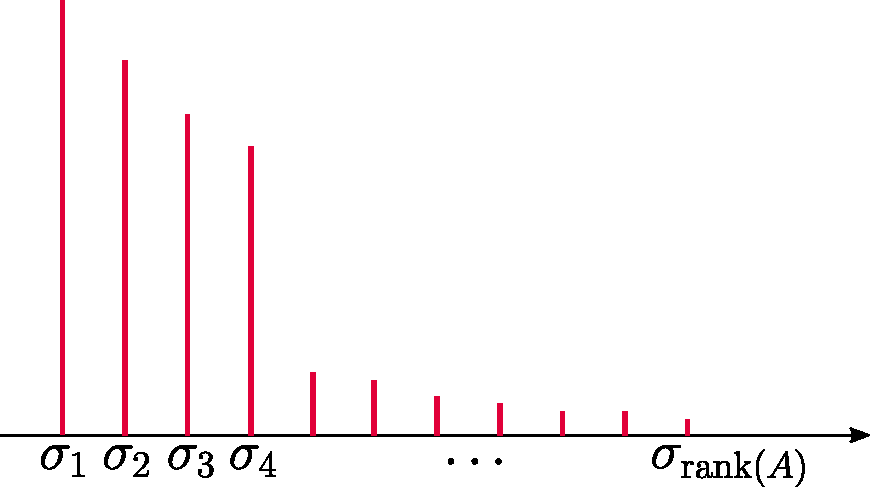
\includegraphics[width = 0.7\linewidth]{figures/elbow.pdf}
	\end{center}
	\caption{Singular values of $A$, ranked in decreasing order.}
	\label{fig:elbow}
\end{figure}

A simple way to chose $k$ is therefore to plot the square singular values as on Figure \ref{fig:elbow} and look for a good cut-off ($k=4$ on Figure \ref{fig:elbow}). Doing so, one captures a fraction
$$
\frac{\sum_{i=1}^k \sigma_i^2}{\sum_{i=1}^{\min(n,d)} \sigma_i^2}
$$
of the total variance.

\paragraph{Should we normalize the dataset?}
It depends, but in general the answer is yes, especially if you have data from eterogeneous types.
Imagine that you have measured the size and the weight of $n$ objects, and stored the information in vectors $a_i= (\text{size of object} \ i \ \text{in cm}, \ \text{weight of object} \ i \text{ in kg})$.
If I change the weighting unit from kilograms to grams, this multiply the variance along the second coordinates by $10^6$, leading to very different principal components.
Normalizing the dataset (i.e.\ dividing the columns of the data matrix by their standard deviation) allows to be unafftected by a change of units.

However, this decreases a lot the variance of that has an high variance and amplify a lot the variance of columns with low variance. Hence you may not always want to normalize the columns.


\subsection{Best-fitting subspace}
Let $a_1, \dots, a_n \in \R^d$ be $n$ points in $d$ dimensions.
We consider the problem of finding the $k$-dimensional subspace (for $k = 1, \dots, n$) that fits ``the best'' these $n$ data points. By ``best'', we mean here the $k$-dimensional subspace $S$ that minimize the sum of the square distances to the $n$ points:
\begin{equation}\label{eq:fit}
	\text{minimize} \ \ \sum_{i=1}^n d(a_i, S)^2 \ \ \text{with respect to} \ S \ \text{subspace of dimension} \ k.
\end{equation}

Let $A$ be the $n \times d$ matrix whose rows are $a_1, \dots, a_n$.
The goal of this section is to prove:
\begin{theorem}\label{th:approx_svd}
	Let $v_1, \dots, v_n$ be right singular vectors of $A$. Then for all $k \in \{1, \dots, n\}$, the subspace $\Span(v_1, \dots, v_k)$ is a solution of \eqref{eq:fit}.
\end{theorem}
In this case we have for all $i \in \{1, \dots, n\}$,
$$
d(a_i, S)^2 = \| a_i - P_{S}(a_i) \|^2 = \|a_i\|^2 - \| P_{S}(a_i) \|^2,
$$
by Pythagorean Theorem (recall that $P_{S}(a_i) \perp (a_i - P_S(a_i))$). Since $v_1$ is of unit norm, $P_{S}(a_i) = \langle v_1, a_i \rangle v_1$, hence:
$$
d(a_i, S)^2 =  \|a_i\|^2 - \langle v_1, a_i \rangle^2.
$$
Minimizing \eqref{eq:fit} is therefore equivalent to maximize
\begin{equation}\label{eq:fit2}
	\sum_{i=1}^n \| P_{S}(a_i) \|^2.
\end{equation}
Let us fix an orthonormal basis $(s_1, \dots, s_k)$ of $S$. Then for all $x \in \R^d$,
$P_S(x)= \langle s_1, x \rangle s_1 + \cdots + \langle s_k, x \rangle s_k$, hence
\begin{equation}\label{eq:fit3}
	\sum_{i=1}^n \| P_{S}(a_i) \|^2 = \sum_{i=1}^n \sum_{j = 1}^k \langle a_i, s_j \rangle^2
	= \| A s_1 \|^2 + \cdots + \| A s_k \|^2,
\end{equation}
Consequently, minimizing \eqref{eq:fit} is equivalent to maximizing \eqref{eq:fit3} over all orthonormal families $(s_1, \dots, s_k)$.
\\

For $k=1$, Proposition \ref{prop:max_svd} tells us that a subspace of dimension $1$ that minimizes \eqref{eq:fit} is $\Span(v_1)$ because
\begin{equation}\label{eq:def_first_singular}
	v_1 = \argmax_{\|v\| = 1} \|A v\|.
\end{equation}
If we now want to solve the problem for $k=2$, a natural candidate for the subspace $S$ would be $S = \Span(v_1, v_2)$ since by Proposition \ref{prop:max_svd}
\begin{equation}\label{eq:def_second_singular}
	v_2 = \argmax_{\|v\| = 1, \, v \perp v_1} \| A v \|.
\end{equation}
We can follow this greedy strategy for $k = 3, \dots, n$, $S = \Span(v_1, \dots, v_k)$ is a natural candidate for being solution of \eqref{eq:fit}.

It is not a priori obvious (except for $k=1$) that $S = \Span(v_1, \dots, v_k)$ is a minimizer of \eqref{eq:fit} over all the subspaces of dimension $k$.
We need the following lemma.

\begin{lemma}\label{lem:svd_rec}
	Let $k \in \{2, \dots, k\}$. Assume that $(v_1, \dots, v_{k-1})$ is an orthonormal family that maximizes \eqref{eq:fit3}.
	Define 
	$$
	v_k = \argmax_{\|v\| = 1, \, v \perp \Span(v_1, \dots, v_{k-1})} \|Av\|.
	$$
	Then $(v_1, \dots, v_{k})$ is an orthonormal family and $\Span(v_1, \dots v_k)$ minimizes \eqref{eq:fit}, i.e.\ $(v_1, \dots, v_{k})$ maximizes \eqref{eq:fit3}.
\end{lemma}
\begin{proof}
	Let $S$ be a subspace of dimension $k$. Let $(w_1, \dots, w_k)$ be an orthonormal basis of $S$ such that $w_{k} \perp \Span(v_1, \dots, v_{k-1})$. By definition of $v_k$,
	we have $\|A w_k \| \leq \| A v_k\|$. 
	We also assumed that $(v_1, \dots, v_k)$ maximizes \eqref{eq:fit3}, so
	$$
	\|A v_1\|^2 + \cdots + \| A v_{k-1} \|^2 \geq
	\|A w_1\|^2 + \cdots+ \| A w_{k-1} \|^2.
	$$
	We conclude that
	$$
	\|A v_1\|^2 + \cdots + \| A v_{k} \|^2 \geq
	\|A w_1\|^2 + \cdots + \| A w_{k} \|^2,
	$$
	so $(v_1, \dots, v_k)$ maximizes \eqref{eq:fit3}.
\end{proof}
\\

Theorem \ref{th:approx_svd} follows then by induction.


\vspace{1cm}
\centerline{\pgfornament[width=7cm]{71}}

%\bibliographystyle{plain}
%\bibliography{./references.bib}
\end{document}
